% =============================================================================
% SECTION 5: PERFORMANCE VERIFICATION & INTERPRETABILITY
% =============================================================================
\section{Performance Verification \& Interpretability}

% ---------------- 20 BEST MODEL PERFORMANCE ----------------
\begin{frame}{Champion Model Metrics Overview}
\centering
\small
\begin{tabular}{lc}
\toprule
\textbf{Evaluation Metric Domain} & \textbf{Champion Value Result} \\
\midrule
Cross-Validation PR-AUC & 0.698 \\
Training Set PR-AUC & 0.797 \\
\textbf{Independent Test Set PR-AUC} & \textbf{0.734} \\
Test Generalization Accuracy & 87.3\% \\
Precision Score (Positive Predictive Value) & 74.9\% \\
Recall Score (Sensitivity) & 56.4\% \\
Balanced F1-Score & 0.643 \\
Area Under the ROC Curve (ROC-AUC) & 0.874 \\
\bottomrule
\end{tabular}
\vspace{0.25cm}
\begin{block}{Generalization Capacity Verification}
The narrow gap between train and test metrics (0.797 vs 0.734) confirms strong model generalization and rules out overfitting.
\end{block}
\end{frame}

% ------------------ 20.5 SLIDE: PRECISION-RECALL CURVE EVALUATION ------------------
\begin{frame}{Model Diagnostics: Precision-Recall Curve}
\begin{columns}[c]
    \column{0.52\textwidth}
        \textbf{Precision-Recall Profile}
        \scriptsize
        \begin{itemize}
            \item \textbf{Test PR-AUC:} \alert{\textbf{0.734}}
            \item Directly matches the evaluation metric targeted during the 5,000-trial Bayesian search.
        \end{itemize}
        \begin{center}
            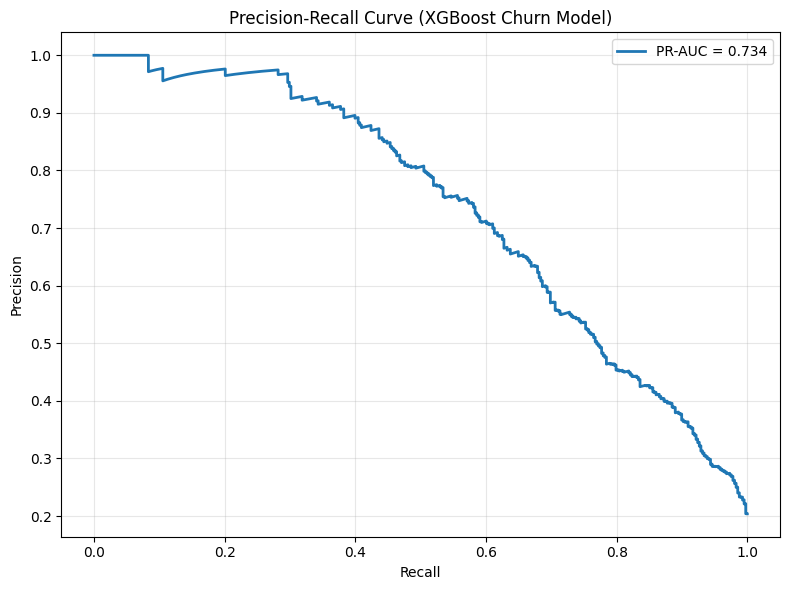
\includegraphics[width=0.9\textwidth]{figures/pr_auc_curve_best_model.png}
        \end{center}
    
    \column{0.45\textwidth}
        \begin{block}{Why PR-AUC Over ROC-AUC?}
            \scriptsize
            With high class imbalance, ROC-AUC can yield an overly optimistic evaluation by incorporating True Negatives. The Precision-Recall curve isolates performance on the minority class by tracking False Positives and False Negatives directly.
        \end{block}
        \begin{exampleblock}{Operational Utility}
            \scriptsize
            Enables business teams to dynamically adjust probability thresholds to balance marketing costs (Precision) against churn detection coverage (Recall).
        \end{exampleblock}
\end{columns}
\end{frame}

% ---------------- 11 FEATURE IMPORTANCE ANALYSIS ----------------
\begin{frame}{Global Feature Importance Rankings}
\scriptsize
\begin{itemize}
    \item \textbf{Feature importance} was extracted from the optimized tree-boosting matrix.
    \item \textbf{Product Portfolio Density} emerged as the primary driver of customer attrition:
    \begin{itemize}
        \item \texttt{NumOfProducts\_2} (25.8\% total attribution)
        \item \texttt{NumOfProducts\_3} (15.4\% total attribution)
        \item \texttt{NumOfProducts\_4} (8.4\% total attribution)
    \end{itemize}
    \item \textbf{Customer Engagement Metrics} contributed significant predictive power:
    \begin{itemize}
        \item \texttt{IsActiveMember} (8.7\% total attribution)
        \item \texttt{Age} (6.6\% total attribution)
    \end{itemize}
    \item \textbf{Geographic Market Location} introduced notable variation:
    \begin{itemize}
        \item \texttt{Geography\_Germany} (7.5\% total attribution)
    \end{itemize}
    \item The top 5 features account for roughly \textbf{66\%} of the model's total predictive attribution. Card type and credit card ownership showed negligible impact.
\end{itemize}
\end{frame}

% ---------------- 13 SHAP ANALYSIS ----------------
\begin{frame}{SHAP Global Interpretability Summary}
\begin{columns}[T]
\column{0.55\textwidth}
\scriptsize
\begin{itemize}
    \item SHAP values map out individual feature impacts on directional churn risk.
    \item \textbf{Risk Accelerators (Increases Churn):}
    \begin{itemize}
    \scriptsize
        \item Advancing customer age profiles.
        \item Portfolios containing 3 or 4 products.
        \item Residence within the German market.
        \item High overall account balances.
    \end{itemize}
    \item \textbf{Risk Decelerators (Reduces Churn):}
    \begin{itemize}
    \scriptsize
        \item Active account membership status.
        \item Portfolios holding exactly 2 products.
        \item Higher baseline customer credit scores.
    \end{itemize}
\end{itemize}

\column{0.45\textwidth}
\centering
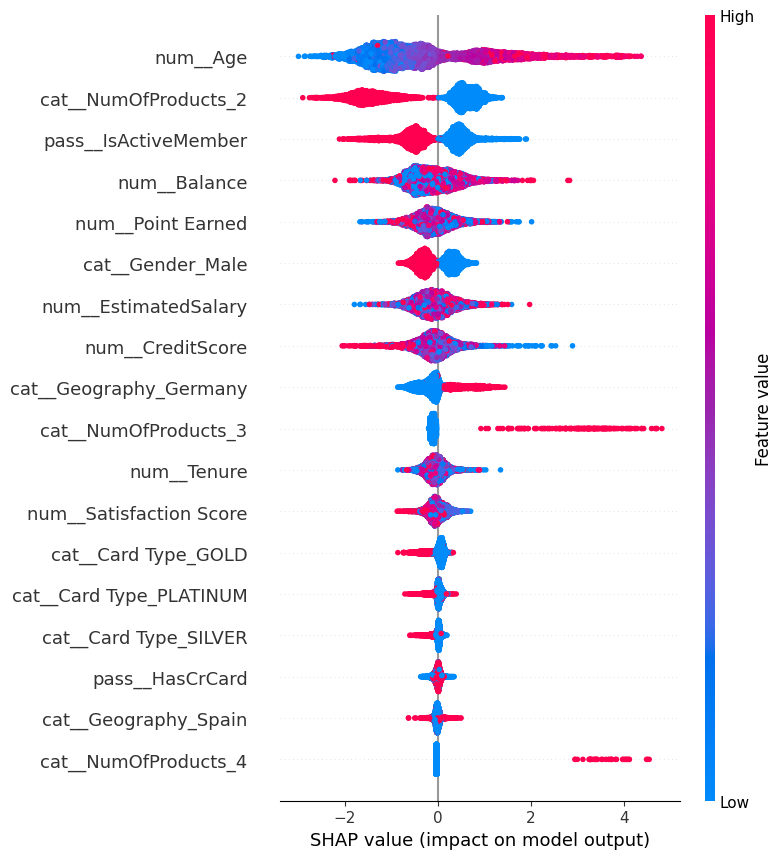
\includegraphics[width=\linewidth]{figures/shap_xgboost.png}
\vspace{0.1cm}
\tiny SHAP beeswarm summary plot for the final XGBoost model.
\end{columns}
\end{frame}

% ---------------- 14 AGE EFFECT ANALYSIS: SHAP Dependence Plot ----------------
\begin{frame}{Age Nonlinearities: SHAP Dependence Plots}
\begin{center}
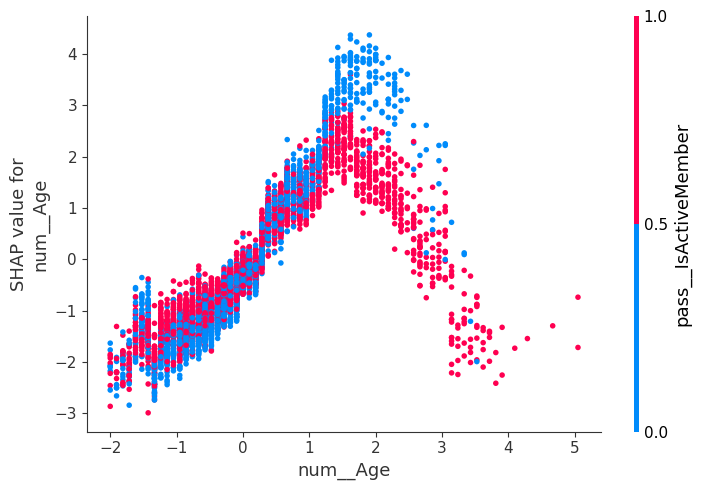
\includegraphics[width=0.70\textwidth]{figures/shap_dependence_num_age.png}
\vspace{0.1cm}
\newline
\tiny \textit{SHAP dependence mapping for \texttt{Age} interacting with \texttt{IsActiveMember}.}
\end{center}
\end{frame}

% ---------------- 15 AGE EFFECT ANALYSIS: Key Findings ----------------
\begin{frame}{Age Dynamics \& Interaction Insights}
\footnotesize
\begin{itemize}
    \item Customer age displays a pronounced non-linear relationship with calculated risk metrics.
    \item A distinct risk transition occurs around normalized age $\approx 2.0$, where SHAP vectors shift from positive to negative.
    \item \textbf{Younger Segments:} Lower overall baseline attrition risk.
    \item \textbf{Middle-Aged Segments:} Peak risk profiles, accelerating attrition probability.
    \item \textbf{Older Segments:} Attrition risk drops back down, showing stable retention behavior.
    \item \textbf{Engagement Interaction Effect:}
    \begin{itemize}
        \item Inactive account status amplifies the middle-age churn spike.
        \item Active account status mitigates risk across all age segments.
    \end{itemize}
\end{itemize}
\begin{block}{Strategic Business Action}
Focus retention marketing directly on middle-aged cohorts, while managing younger and older segments as low-risk baselines.
\end{block}
\end{frame}

% ---------------- 22 FEATURE IMPORTANCE ----------------
\begin{frame}{Global Impact Drivers}
\begin{columns}[T]
\column{0.50\textwidth}
\begin{block}{Global SHAP Interpretations}
    \scriptsize
SHAP values isolate the absolute directional risk contribution of every feature across all observations.
\end{block}
\begin{itemize}
    \scriptsize
    \item \textbf{Product Portfolio Structure:} Total product count serves as the model's primary prediction anchor.
    \item \textbf{Financial Profile Interactions:} Credit score combined with age provides a refined risk signal.
    \item \textbf{Engagement Footprints:} Inactivity paired with high account balances flags high-risk accounts.
    \item \textbf{Low-Impact Variables:} Estimated salary and card tier labels show minimal predictive value.
\end{itemize}

\column{0.58\textwidth}
\centering
\vspace{0.4cm}
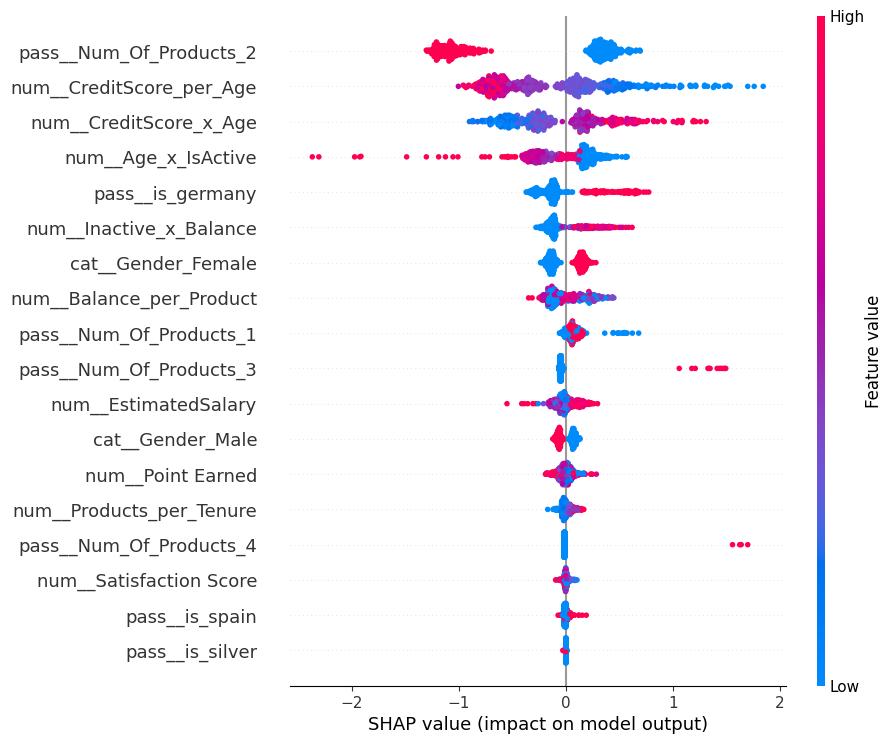
\includegraphics[width=\textwidth]{figures/final_model_shap.png}
\end{columns}
\end{frame}

% ---------------- 23 INTERPRETABILITY ----------------
\begin{frame}{Local Interpretability: Customer Risk Case Study}
\begin{columns}[T]
\column{0.55\textwidth}
\textbf{High-Risk Account Breakdown}
\begin{itemize}
    \item \textbf{Risk Amplifiers:}
    \begin{itemize}
    \scriptsize
        \item High CreditScore $\times$ Age interaction.
        \item Unfavorable CreditScore-to-Age ratio.
        \item High balance on an inactive account.
    \end{itemize}
    \item \textbf{Risk Mitigators:}
    \begin{itemize}
    \scriptsize
        \item Favorable balance-to-product ratio.
        \item Substantial reward point accrual.
    \end{itemize}
\end{itemize}
\textbf{Value to Business:}
Provides transparent, auditable explanations to justify individual customer retention actions.

\column{0.50\textwidth}
\scriptsize
\begin{block}{SHAP Local Waterfall Implementations}
Waterfall plots break down exactly how specific features shift an individual prediction away from the baseline expected value.
\end{block}
\centering
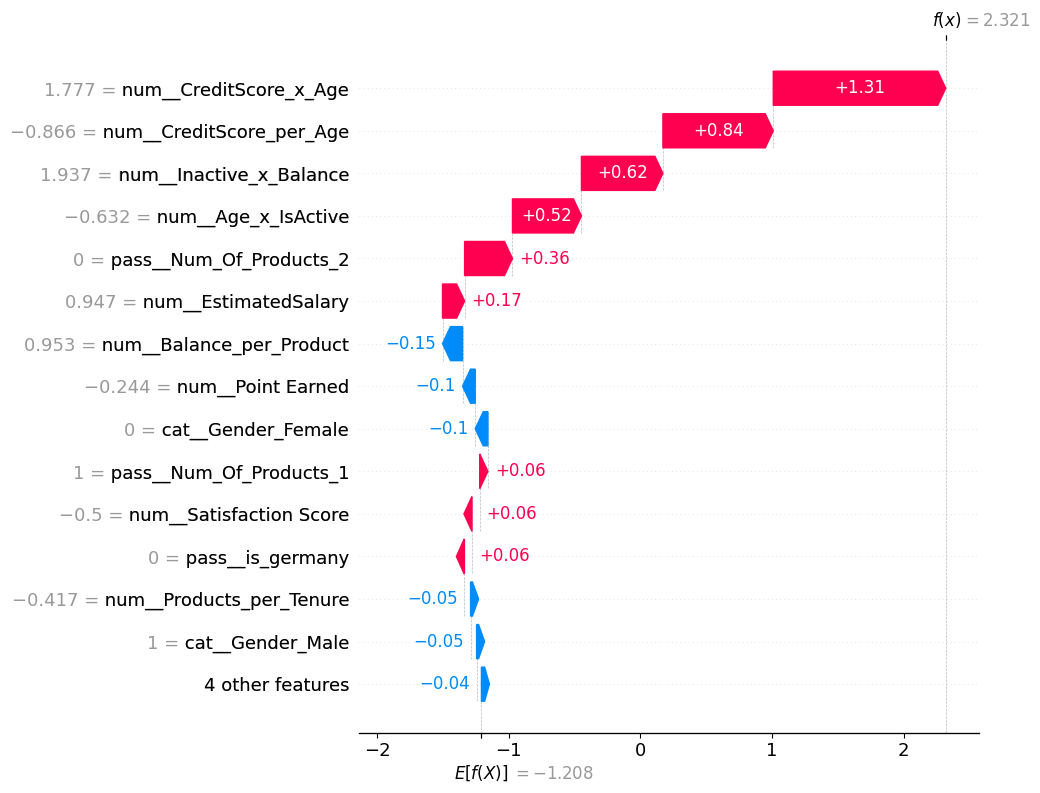
\includegraphics[width=\textwidth]{figures/explain_customer_0.png}
\end{columns}
\end{frame}

% ---------------- 12 BUSINESS INSIGHTS ----------------
\begin{frame}{Key Strategic Business Insights}
\scriptsize
\begin{itemize}
    \item \textbf{Product Portfolio Alignment:} Product counts are the strongest indicator of churn, with multi-product combinations driving anomalies.
    \item \textbf{Engagement Leverage:} Active account membership remains the single most reliable hedge against customer attrition.
    \item \textbf{Geographic Disparities:} localized operational conditions in the German market require customized regional retention strategies.
    \item \textbf{Age Demographics:} Risk centers on middle-aged segments, requiring age-tailored outreach.
\end{itemize}
\scriptsize
\begin{exampleblock}{Priority Core Initiatives}
    \begin{enumerate}
        \item Focus campaigns on re-engaging inactive accounts.
        \item Optimize multi-product account groupings to prevent portfolio friction.
        \item Deploy specialized retention strategies for high-risk regional markets.
    \end{enumerate}
\end{exampleblock}
\end{frame}